\documentclass[tikz,border=3mm]{standalone}
\usepackage[T1]{fontenc}
\usepackage{helvet}                       % IEEE-recommended Helvetica
\renewcommand{\familydefault}{\sfdefault}
\usepackage{amsmath,amssymb}
\usepackage{tikz}
\usetikzlibrary{shapes.geometric, positioning, decorations.pathreplacing,
                arrows.meta, calc}

\begin{document}
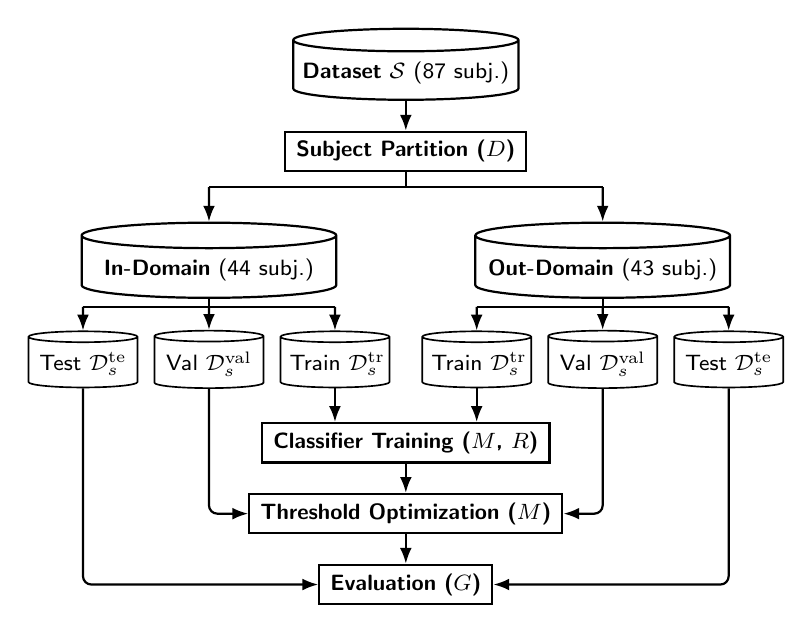
\begin{tikzpicture}[
  every node/.style={font=\sffamily\footnotesize},
  >=Latex,
  %% Pipeline node styles — font/padding aligned with framework_general
  db/.style={draw, thick, cylinder, cylinder uses custom fill,
    cylinder body fill=white, shape border rotate=90, aspect=0.10,
    minimum width=2.6cm, minimum height=0.7cm, align=center,
    font=\sffamily\footnotesize},
  dbsm/.style={draw, semithick, cylinder, cylinder uses custom fill,
    cylinder body fill=white, shape border rotate=90, aspect=0.10,
    minimum width=1.35cm, minimum height=0.5cm, text width=1.15cm,
    align=center, font=\sffamily\footnotesize},
  pbox/.style={draw, thick,
    align=center, fill=white,
    minimum height=0.5cm,
    inner xsep=4pt, inner ysep=2pt,
    font=\sffamily\footnotesize},
  arr/.style ={-{Latex[length=2mm, width=1.5mm]}, thick},
]

%% =========================================================
%% UPPER HALF — data partitioning
%% =========================================================
%% ROW 0 — Dataset
\node[db] (dataset) at (0,0)
  {\textbf{Dataset}~$\mathcal{S}$ (87 subj.)};

%% ROW 1 — Subject Partition (parameterised by D)
\node[pbox] (dsplit) at (0,-1.00)
  {\textbf{Subject Partition ($D$)}};
\draw[arr] (dataset.south) -- (dsplit.north);

%% ROW 2 — In-Domain / Out-Domain cylinders
\node[db, text width=3.0cm] (src) at (-2.5,-2.5)
  {\textbf{In-Domain}~(44 subj.)};
\node[db, text width=3.0cm] (tgt) at ( 2.5,-2.5)
  {\textbf{Out-Domain}~(43 subj.)};

\coordinate (forkMid) at ($(dsplit.south)!.3!(src.north)$);
\coordinate (forkC) at (0,0 |- forkMid);
\coordinate (forkL) at (-2.5,0 |- forkMid);
\coordinate (forkR) at ( 2.5,0 |- forkMid);
\draw[thick] (dsplit.south) -- (forkC);
\draw[thick] (forkL) -- (forkR);
\draw[arr] (forkL) -- (src.north);
\draw[arr] (forkR) -- (tgt.north);

%% ROW 3 — Per-subject 70/15/15 split
\node[dbsm] (test_s)  at (-4.1,-3.7) {Test~$\mathcal{D}_s^{\mathrm{te}}$};
\node[dbsm] (val_s)   at (-2.5,-3.7) {Val~$\mathcal{D}_s^{\mathrm{val}}$};
\node[dbsm] (train_s) at (-0.9,-3.7) {Train~$\mathcal{D}_s^{\mathrm{tr}}$};

\coordinate (forkS) at ($(src.south)!.25!(test_s.north)$);
\draw[semithick] (src.south) -- (-2.5,0 |- forkS);
\draw[semithick] (-4.1,0 |- forkS) -- (-0.9,0 |- forkS);
\draw[arr] (-4.1,0 |- forkS) -- (test_s.north);
\draw[arr] (-2.5,0 |- forkS) -- (val_s.north);
\draw[arr] (-0.9,0 |- forkS) -- (train_s.north);

\node[dbsm] (train_t) at (0.9,-3.7) {Train~$\mathcal{D}_s^{\mathrm{tr}}$};
\node[dbsm] (val_t)   at (2.5,-3.7) {Val~$\mathcal{D}_s^{\mathrm{val}}$};
\node[dbsm] (test_t)  at (4.1,-3.7) {Test~$\mathcal{D}_s^{\mathrm{te}}$};

\coordinate (forkT) at ($(tgt.south)!.25!(test_t.north)$);
\draw[semithick] (tgt.south) -- (2.5,0 |- forkT);
\draw[semithick] (0.9,0 |- forkT) -- (4.1,0 |- forkT);
\draw[arr] (0.9,0 |- forkT) -- (train_t.north);
\draw[arr] (2.5,0 |- forkT) -- (val_t.north);
\draw[arr] (4.1,0 |- forkT) -- (test_t.north);

%% =========================================================
%% LOWER HALF — three ML-pipeline blocks
%% =========================================================
%% ROW 4 — Classifier Training
\node[pbox] (cls) at (0,-4.70)
  {\textbf{Classifier Training}~\textbf{($M$, $R$)}};
\draw[arr] (train_s.south) -- (train_s.south |- cls.north);
\draw[arr] (train_t.south) -- (train_t.south |- cls.north);

%% ROW 5 — Threshold Optimization
\node[pbox] (thr) at (0,-5.60)
  {\textbf{Threshold Optimization}~\textbf{($M$)}};
\draw[arr] (cls.south) -- (thr.north);

%% ROW 6 — Evaluation
\node[pbox] (eval) at (0,-6.50)
  {\textbf{Evaluation}~\textbf{($G$)}};
\draw[arr] (thr.south) -- (eval.north);

%% Val / Test trunks
\draw[arr, rounded corners=3pt]
  (val_s.south) -- (-2.5,-5.60) -- (thr.west);
\draw[arr, rounded corners=3pt]
  (val_t.south) -- ( 2.5,-5.60) -- (thr.east);
\draw[arr, rounded corners=3pt]
  (test_s.south) -- (-4.1,-6.50) -- (eval.west);
\draw[arr, rounded corners=3pt]
  (test_t.south) -- ( 4.1,-6.50) -- (eval.east);

\end{tikzpicture}
\end{document}
